% !Mode:: "TeX:UTF-8"
% !TeX encoding = UTF8
 
\documentclass[12pt,border=8pt]{standalone}

% For automata drawings
\usepackage{tikz}
\usepackage{pgf}
\usetikzlibrary{arrows}

\begin{document}
 
  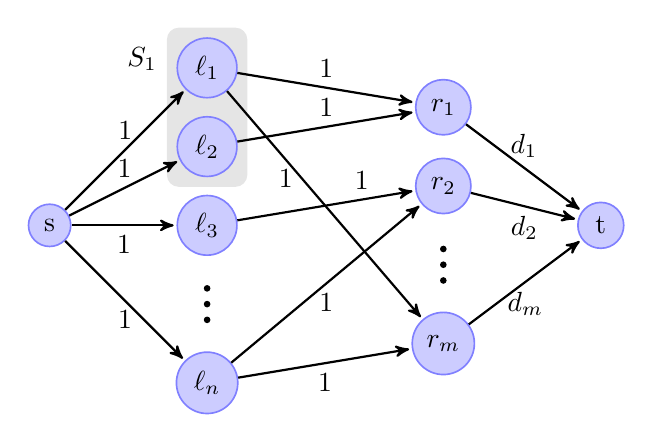
\begin{tikzpicture}[
    % type of arrow head
    >=stealth',
    % keep arrow head from touching the surface
    shorten >= 1pt,
    % automatic node positioning
    auto,
    %
    node distance=2cm,
    % line thickness
    semithick,
    bend angle=10,
    graybox/.style = {draw=gray!20, fill=gray!20, rounded corners},
    line/.style = {->, draw=black, thick},
    box/.style = {circle, draw=blue!50, fill=blue!20, minimum size=4mm}
    ]

    \coordinate (S) at (-5cm, 0cm);

    \coordinate (S1) at (-3cm, 2cm);
    \coordinate (S2) at (-3cm, 1cm);
    \coordinate (S3) at (-3cm, 0cm);
    \coordinate (S4) at (-3cm, -2cm);

    \coordinate (M1) at (0cm, 1.5cm);
    \coordinate (M2) at (0cm,  .5cm);
    \coordinate (M3) at (0cm,-1.5cm);

    \coordinate (T) at (2cm, 0cm);

    \node (BBox) [graybox, minimum width=1cm, minimum height=2cm] at (-3cm, 1.5cm) {};
    \node [left] at (BBox.130) {$S_1$};

     % nodes
    \node (Sbox)  [box] at (S)  {s};
    \node (Sbox1) [box] at (S1) {$\ell_1$};
    \node (Sbox2) [box] at (S2) {$\ell_2$};
    \node (Sbox3) [box] at (S3) {$\ell_3$};
    \node (Sbox4) [box] at (S4) {$\ell_n$};

    \node (Mbox1) [box] at (M1) {$r_1$};
    \node (Mbox2) [box] at (M2) {$r_2$};
    \node (Mbox3) [box] at (M3) {$r_m$};

    \node (Tbox) [box] at (T) {t};

    \fill [black] (-3cm,  -.8cm) circle (1.2pt);
    \fill [black] (-3cm,   -1cm) circle (1.2pt);
    \fill [black] (-3cm, -1.2cm) circle (1.2pt);

    \fill [black] (0cm, -.3cm) circle (1.2pt);
    \fill [black] (0cm, -.5cm) circle (1.2pt);
    \fill [black] (0cm, -.7cm) circle (1.2pt);


    % edges
    \path[line] (Sbox) -- node [above] {1} (Sbox1);
    \path[line] (Sbox) -- node [above] {1} (Sbox2);
    \path[line] (Sbox) -- node [below] {1} (Sbox3);
    \path[line] (Sbox) -- node [below] {1} (Sbox4);

    \path[line] (Sbox1) -- node [above] {1} (Mbox1);
    \path[line] (Sbox2) -- node [above] {1} (Mbox1);

    \path[line] (Sbox3) -- node [above, pos=.7] {1} (Mbox2);

    \path[line] (Sbox1) -- node [below, pos=.3] {1} (Mbox3);

    \path[line] (Sbox4) -- node [below] {1} (Mbox2);
    \path[line] (Sbox4) -- node [below] {1} (Mbox3);

    \path[line] (Mbox1) -- node [above] {$d_1$} (Tbox);
    \path[line] (Mbox2) -- node [below] {$d_2$} (Tbox);
    \path[line] (Mbox3) -- node [below] {$d_m$} (Tbox);
   \end{tikzpicture}
 
\end{document}